\chapter{Proverb 9}

\begin{figure}
  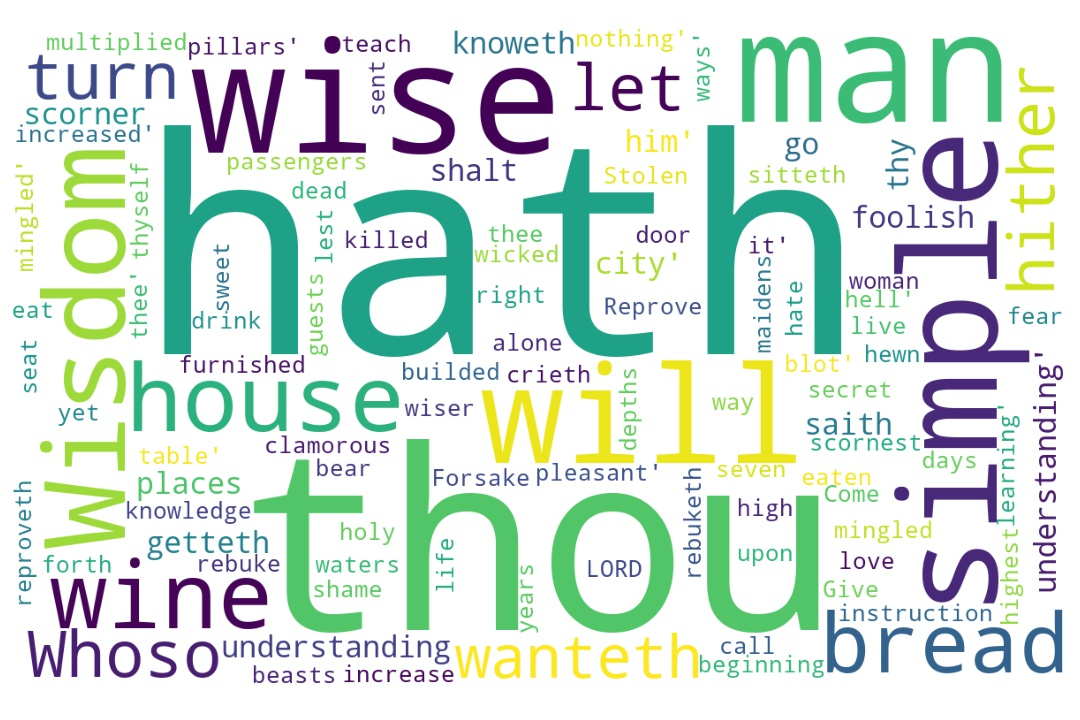
\includegraphics[width=\linewidth]{20OT-Proverbs/Proverb9-WordCloud.jpg}
  \caption{Proverb 9 Word Cloud}
  \label{fig:Proverb 9 Word Cloud}
\end{figure}


\marginpar{\scriptsize \centering \fcolorbox{bone}{lime}{\textbf{WISDOM: THE GOOD CHOICE}}\\ (Proverb 9:1-18) \begin{compactenum}[I.][8]
\item \textbf{Builds} a Life \index[scripture]{Proverbs!Pro 09:01}(Pro 9:1)
\item Has a \textbf{Banquet} \index[scripture]{Proverbs!Pro 09:02}(Pro 9:2)
\item Gives out \textbf{Bread} \index[scripture]{Proverbs!Pro 09:05}(Pro 9:5)
\item Has \textbf{Blessings} \index[scripture]{Proverbs!Pro 09:09}(Pro 9:9)
\item Was there from the \textbf{Beginning} \index[scripture]{Proverbs!Pro 09:10}(Pro 9:10)
\item Provides Lasting \textbf{Benefits} \index[scripture]{Proverbs!Pro 09:11}(Pro 9:11)
\item Is \textbf{Betrayed} \index[scripture]{Proverbs!Pro 09:13}(Pro 9:13)
\end{compactenum}}

\marginpar{\scriptsize \centering \fcolorbox{bone}{yellow}{\textbf{WISDOM AT WORK}}\\ (Proverb 9:1-18) \begin{compactenum}[I.][8]
    \item \textbf{Builds a House} \index[scripture]{Proverbs!Pro 09:01}(Pro 9:1)
    \item \textbf{Hews out Pillars} \index[scripture]{Proverbs!Pro 09:01}(Pro 9:1)
    \item \textbf{Kills her Beats} \index[scripture]{Proverbs!Pro 09:02}(Pro 9:2)
    \item \textbf{Mingles Her Wine} \index[scripture]{Proverbs!Pro 09:02}(Pro 9:2)
    \item \textbf{Furnishes her Table} \index[scripture]{Proverbs!Pro 09:02}(Pro 9:2)
    \item \textbf{Sends forthe her Maidens} \index[scripture]{Proverbs!Pro 09:03}(Pro 9:3)
    \item \textbf{Cries from the High Places} \index[scripture]{Proverbs!Pro 09:03}(Pro 9:3)
\end{compactenum}}

\marginpar{\scriptsize \centering \fcolorbox{bone}{black}{\textbf{\textcolor[cmyk]{0,0,0,0}{LOOKING FOR WISDOM}}}\\ (Proverb 9) 
\begin{compactenum}[I.][8]
    \item The \textbf{Rendering of Wisdom} \index[scripture]{Proverbs!Pro 09:01}(Pro 9:1) 
   \item The \textbf{Reaction to Wisdom} \index[scripture]{Proverbs!Pro 09:09}(Pro 9:9) 
    \item The \textbf{Reach for Wisdom} \index[scripture]{Proverbs!Pro 09:10}(Pro 9:10) 
    \item The \textbf{Road to Wisdom} \index[scripture]{Proverbs!Pro 09:11}(Pro 9:11) 
    \item The \textbf{Rejection of Wisdom} \index[scripture]{Proverbs!Pro 09:13}(Pro 9:13) 
    \item Man's \textbf{Regard \& Reverence for Foolishness} \index[scripture]{Proverbs!Pro 09:14}(Pro 9:14) 
    \item A \textbf{Reunion of Fools} \index[scripture]{Proverbs!Pro 09:15}(Pro 9:15) 
\end{compactenum}}

\footnote{\textcolor[cmyk]{0.99998,1,0,0}{\hyperlink{TOC}{Return to end of Table of Contents.}}}\footnote{\href{https://audiobible.com/bible/proverbs_9.html}{\textcolor[cmyk]{0.99998,1,0,0}{Proverbs Audio}}}\textcolor[cmyk]{0.99998,1,0,0}{Wisdom hath \fcolorbox{bone}{lime}{builded her house}, she hath hewn out her seven pillars:}\footnote{\textbf{1 Kings 8:27} - But will God indeed dwell on the earth? behold, the heaven and heaven of heavens cannot contain thee; how much less this house that I have builded?} 
[2] \textcolor[cmyk]{0.99998,1,0,0}{She hath killed her beasts; she hath mingled her wine; she hath also \fcolorbox{bone}{lime}{furnished} her table.}
[3] \textcolor[cmyk]{0.99998,1,0,0}{She hath sent forth her maidens: she crieth upon the highest places of the city,}
[4] \textcolor[cmyk]{0.99998,1,0,0}{Whoso \emph{is} simple, let him turn in hither: \emph{as} \emph{for} him that wanteth \fcolorbox{bone}{MYGOLD}{understanding}, she saith to him,}
[5] \textcolor[cmyk]{0.99998,1,0,0}{Come, \fcolorbox{bone}{lime}{eat of my} \fcolorbox{bone}{lime}{bread}, and drink of the wine \emph{which} I have mingled.}
[6] \textcolor[cmyk]{0.99998,1,0,0}{Forsake the foolish, and live; and go in the way of \fcolorbox{bone}{MYGOLD}{understanding}.}
[7] \textcolor[cmyk]{0.99998,1,0,0}{He that reproveth a scorner getteth to himself shame: and he that rebuketh a wicked \emph{man} \emph{getteth} himself a blot.}
[8] \textcolor[cmyk]{0.99998,1,0,0}{Reprove not a scorner, lest he hate thee: rebuke a wise man, and he will love thee.}
[9] \textcolor[cmyk]{0.99998,1,0,0}{Give \emph{instruction} to a wise \emph{man}, and he will \fcolorbox{bone}{lime}{be yet wiser}: teach a just \emph{man}, and he will increase in learning.}
[10] \textcolor[cmyk]{0.99998,1,0,0}{The fear of the LORD \emph{is} the \fcolorbox{bone}{lime}{beginning of wisdom}: and the knowledge of the holy \emph{is} \fcolorbox{bone}{MYGOLD}{understanding}.}
[11] \textcolor[cmyk]{0.99998,1,0,0}{For by me thy days shall be multiplied, and the years of thy life shall be \fcolorbox{bone}{lime}{increased}.}
[12] \textcolor[cmyk]{0.99998,1,0,0}{If thou be wise, thou shalt be wise for thyself: but \emph{if} thou scornest, thou alone shalt bear \emph{it}.}
[13] \textcolor[cmyk]{0.99998,1,0,0}{A foolish woman \emph{is} clamorous: \emph{she} \emph{is} simple, and \fcolorbox{bone}{lime}{knoweth nothing}.}
[14] \textcolor[cmyk]{0.99998,1,0,0}{For she sitteth at the door of her house, on a seat in the high places of the city,}
[15] \textcolor[cmyk]{0.99998,1,0,0}{To call passengers who go right on their ways:}
[16] \textcolor[cmyk]{0.99998,1,0,0}{Whoso \emph{is} simple, let him turn in hither: and \emph{as} \emph{for} him that wanteth \fcolorbox{bone}{MYGOLD}{understanding}, she saith to him,}
[17] \textcolor[cmyk]{0.99998,1,0,0}{Stolen waters are sweet, and bread \emph{eaten} in secret is pleasant.}
[18] \textcolor[cmyk]{0.99998,1,0,0}{But he knoweth not that the dead \emph{are} there; \emph{and} \emph{that} her guests \emph{are} in the depths of hell.}


